\documentclass[12pt]{article}

\usepackage[margin=1in]{geometry}
	%changes default margins

\usepackage{setspace}
\singlespacing
	%\singlespacing,\onehalfspacing,\doublespacing can be set and everything thereafter will use that spacing. You can switch within the document as often as you wish
	
\usepackage{parskip}
%changes paragraphs to have an extra space and new indentation with paragraphs, rather than indenting every new paragraph. This is completely a stylistic choice and neither is better than the other.


\usepackage{mathtools,amssymb} %useful math stuff. there are a lot of ams* packages. If you have a math need, it's probably in there

	
	
%\usepackage{natbib}
%\usepackage{biblatex} %natbib is older and available from almost all journals, biblatex is not, but biblatex has more flexibility and options.

%\usepackage[natbib=true]{biblatex} %this often works and requires minimal changes 

%for biblatex you write \textcite{citekey} and \parencite{citekey}
%for natbib you write \citet{citekey} and \citep{citekey}. Please avoid using \cite{} since you won't control whether it's parenthetical, but you are responsible for whether you use something in text or parenthetically.
%for \usepackage[natbib=true]{biblatex} you follow the natbib style and you won't have to perform search/replaces in your document, you would only need to change the package call and bibliography call.

\usepackage{natbib}
\bibliographystyle{chicago}

%other useful packages
\usepackage{graphicx} %for including images including pdf
\usepackage{booktabs} % for tables
\usepackage{siunitx} % for longitude and latitude degrees


\title{Using Machine-Learning Methods to Improve Air Temperature prediction from the Outputs of a Numerical Weather Prediction
Model}
\date{\today}

\author{Anonymized}

\begin{document}
	
\maketitle
	
\section*{Abstract}

This study explores the utilization of machine-learning techniques to enhance air temperature predictions derived from the outputs of a Numerical Weather Prediction (NWP) model. By leveraging historical climatological data and reanalysis products, we aim to address inherent biases and inaccuracies present in NWP model outputs, particularly in regions with complex atmospheric dynamics. The research focuses on developing robust machine-learning models capable of calibrating NWP model outputs to improve the accuracy of surface temperature estimates. Through rigorous variable selection, cross-validation, and model evaluation methodologies, we assess the performance and generalization capability of the proposed models. The findings provide valuable insights into the effectiveness of machine-learning approaches in augmenting the predictive capability of NWP models, with implications for various applications including weather forecasting, climate modeling, and environmental management.

\section{Introduction}

Numerical Weather Prediction (NWP) models play a pivotal role in modern meteorology by providing forecasts of atmospheric conditions based on mathematical simulations of physical processes. Despite significant advancements in NWP modeling techniques, inherent biases and inaccuracies persist in model outputs, particularly in regions characterized by complex atmospheric dynamics. These discrepancies pose challenges for accurate weather prediction and hinder the reliability of NWP model outputs for various applications.

To address these challenges, this study investigates the application of machine-learning methods to enhance the accuracy and reliability of air temperature predictions derived from NWP model outputs. By leveraging historical climatological data and reanalysis products, we aim to develop robust machine-learning models capable of calibrating NWP model outputs to improve the accuracy of surface temperature estimates. The research focuses on assessing the performance and generalization capability of the proposed models through rigorous variable selection, cross-validation, and model evaluation methodologies.

Through this research, we aim to contribute to the advancement of weather prediction techniques by exploring innovative approaches to calibrate and refine NWP model outputs. By improving the accuracy and reliability of surface temperature predictions, our findings have implications for various applications, including weather forecasting, climate modeling, environmental monitoring, and decision-making in sectors such as agriculture, energy, and disaster management.

\section{Literature review}

An atmospheric reanalysis involves retrospectively describing the atmospheric state by assimilating observations into an atmospheric model simulation using data assimilation techniques. Reanalysis products provide a consistent and continuous description of the atmospheric state over a relatively long period, typically spanning 40 to 70 years, and are particularly valuable in regions where observational data are sparse (\cite{Jung2016}). These products are widely used to estimate past and present atmospheric conditions over the world (\cite{Large2009,Tsujino2018}).

However, due to the limitation of the implemented numerical models, errors may occur, especially in regions with shallow atmospheric boundary layers and temperature inversions, which are challenging features for models to simulate accurately (\cite{Zampieri2018}). Previous studies have identified significant surface temperature biases in most reanalysis products over the world, primarily attributed to inaccuracies in representing the snow and sea ice state. Future reanalysis versions are expected to address these deficiencies by incorporating fully coupled modeling systems and assimilating new types of near-surface observations. 

This study explores the use of machine learning algorithms to correct the surface temperature data of GDAS/FNL. GDAS/FNL stands for Global Data Assimilation System/Final Analysis, which is operated by the National Centers for Environmental Prediction (NCEP) in the United States to generate global atmospheric analysis data. GDAS/FNL data are produced by assimilating data from various observational sources (such as satellite observations, surface stations, aircraft probes, etc.) using data assimilation techniques to provide high-quality meteorological field data for various regions worldwide. 

Many scholars have conducted corrections on reanalysis data by machine learning algorithms. \cite{Zampieri2023} used machine learning to correct various datasets and the correction leads on average to a 27\% temperature bias reduction for ERA5 and 7\% for JRA-55 if compared to independent in situ observations from the MOSAiC campaign (respectively, 32\% and 10\% under clear-sky conditions). \cite{Hou2022} applied LDA correction to ERA5 data, and compared with ERA5 and station observation data, the results show that the root mean square error can be reduced by 2\%–4\% and the correlation coefficient can be increased by 1\%–5\% for different lead times, with the most distinct improvement effect for the medium-term forecast time.

In our study, the correction model is trained using surface observations. This approach aims to improve the realism of surface temperature estimates over Toronto regions. 

\section{Data and methodology}

In this project, we explored three different dataset, the first two are combined used as our correction methodologies for a global weather model using local data, the third dataset is a local dataset to test the time series forcasting model on a local scale.

\subsection{Data}

The following sections present some brief introductories of each data set we used, the key variables included in each data set, and how we do the data preprocessing.

\subsubsection{NCEP}

The NCEP (National Centers for Environmental Prediction) Global Forecast System (GFS) model is a numerical weather prediction system operated by the National Weather Service (NWS) of the United States. It is one of the major global models used for weather forecasting worldwide. The GFS model utilizes complex mathematical equations to simulate the behavior of the atmosphere and predict future weather conditions.

The GFS model generates forecasts for a wide range of atmospheric variables including temperature, humidity, wind speed and direction, precipitation, and pressure at various levels of the atmosphere (As shown in Table~\ref{tab:GFS}). These forecasts are produced for different time ranges ranging from short-term forecasts (hours to a few days) to medium-range forecasts (up to two weeks or more).

\begin{table}[htbp]
    \centering
    \caption{NCEP GFS Model Key Features}
    \begin{tabular}{@{}ll@{}}
        \toprule
        \textbf{Parameter} & \textbf{Description} \\
        \midrule
        Air Temperature & Temperature of the air in degrees Celsius or Fahrenheit \\
        Wind Speed & Speed of the wind in meters per second or miles per hour \\
        Precipitation & Amount of precipitation in millimeters or inches \\
        Relative Humidity & Percentage of moisture in the air relative to saturation \\
        Pressure & Atmospheric pressure in hectopascals or millibars \\
        Cloud Cover & Fraction of the sky covered by clouds \\
        \bottomrule
    \end{tabular}
    \label{tab:GFS}
\end{table}

The model ingests observational data from various sources including weather stations, satellites, radar, and aircraft to initialize the simulation of the atmosphere. It then uses sophisticated numerical techniques to solve the equations of fluid motion, thermodynamics, and other physical processes that govern atmospheric behavior.

The output from the GFS model is used by meteorologists and weather forecasters to generate weather forecasts, issue warnings for severe weather events, and provide guidance for various sectors including agriculture, transportation, energy, and emergency management.

In our model, our predictions is the corrections of air temperature output of GFS model. GFS model simulate atmospheric processes on a grid system. The precision of the grid is determined by the spacing of grid points in both horizontal and vertical dimensions. Higher precision grids have smaller spacing between grid points, allowing for more detailed representation of atmospheric features and processes. In our case, we selected a specific grid with 1 degree Based on that value and the locally collected data, we train a calibration model to improve the local air temperature prediction.

\subsubsection{DACCD}

For local temperature data, we use data from the Digital Archive of Canadian Climatological Data (DACCD). It is a comprehensive repository of historical climatological information specific to Canada. Managed by Environment and Climate Change Canada (ECCC), the DACCD houses a vast collection of meteorological data spanning several decades, including observations of temperature, precipitation, wind patterns, atmospheric pressure, and other relevant climatic variables (As shown in Table~\ref{tab:DACCD}). This data is sourced from various observation stations, weather monitoring networks, and research initiatives conducted throughout Canada's vast geographic landscape.

\begin{table}[htpb]
	\centering
	\caption{Key features in the DACCD dataset}
	\label{tab:DACCD}
	\begin{tabular}{lll}
	\toprule
	 Variables & Symbol & Unit\\
	\midrule
	Longitude & x & deg\\
	Latitude & y & deg\\
	Daily mean temperature & Mean Temp & degC\\
	Daily max temperature & Max Temp & degC\\
	Daily min temperature & Min Temp & degC\\
	Daily total rainfall & Total Rain & mm\\
	Daily total snowfall & Total Snow & cm\\
	Daily total precip & Total Precip & mm\\
	Snow on the Ground& Snow on Grnd & cm\\
	Direction of extreme gust & Dir of Max Gust & 10's of deg\\
	Speed of extreme gust & Spd of Max Gust & km/h\\
	\bottomrule
	\end{tabular}
\end{table}

The climatological data in the DACCD dataset are stored at five distinct intervals: minutely, every fifteen minutes, hourly, daily, or monthly. For this project, we specifically utilize the daily data for analysis and modeling purposes.


Weather station selection: The blue box in Figure~\ref{Fig:stations} shows one grid in the GFS model. It bounds a latitude from \ang{43.00} N to \ang{44.00}N, and a longitude from \ang{-79.00} E to \ang{-80.00} E. Using this boundary, we can select all weather stations whose location falls into this grid. In total we got 291 weather stations. However, since the data set contains all historical weather station records from the 19th centry, it is obvious that not all stations are in operation now. Moreover, we want to collect the weather data for a period of time so that we can have enough data to train our model. Therefore, we filtered out all operating weather stations from year 2016 to 2023 in the grid, which end up with only 11 stations marked in red numbers in Figure~\ref{Fig:stations}. Those red numbers are the station ID of each weather station.

\begin{figure}[htpb]
	\centering
	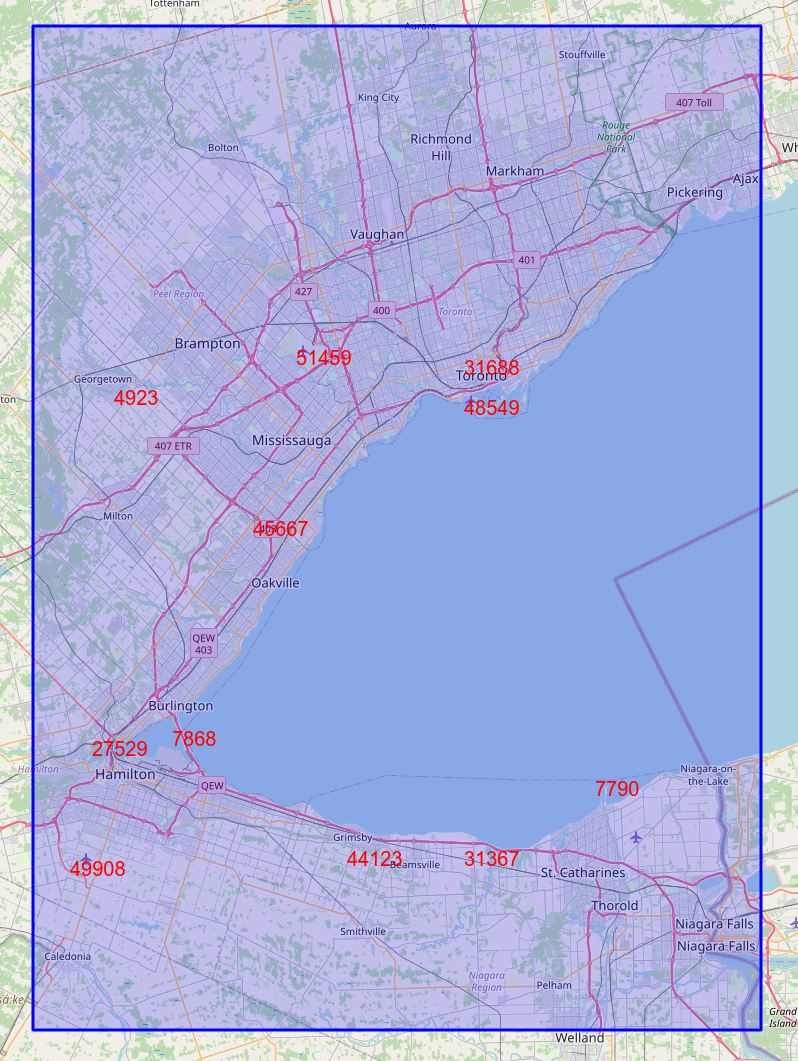
\includegraphics[width=0.8\textwidth]{pic/stations-ID.png}
	\caption{Weather stations used in this project}
	\label{Fig:stations}
\end{figure}

\subsubsection{Jena Weather dataset}

The Max-Planck-Institute for Biogeochemistry, located in Jena, Germany, provides a comprehensive weather dataset encompassing various meteorological parameters. This dataset spans a significant period, with measurements collected every 10 minutes, starting from the year 2003. It comprises 14 distinct features, including crucial metrics such as air temperature, atmospheric pressure, and humidity. Details shown in Table~\ref{tab:Jena}.

To ensure computational efficiency and focus on a specific timeframe, we will narrow down our analysis to the data collected between the years 2009 and 2016. This time span offers a substantial duration for observation while maintaining computational manageability.

\begin{table}[htpb]
	\centering
	\caption{Key features within the Jena dataset}
	\label{tab:Jena}
	\begin{tabular}{lll}
	\toprule
	Variables & Symbol & Unit\\
	\midrule
	Atmospheric pressure & p & mbar\\
	Air temperature & T & degC\\
	Potential temperature & Tpot & K\\
	Dew point temperature & Tdew & degC\\
	Relative humidity & rh & \%\\
	Saturation water vapor pressure & VPmax & mbar\\
	Actual water vapor pressure & VPact & mbar\\
	Water vapor pressure deficit & VPdef & mbar\\
	Specific humidity & sh & g/kg\\
	Water vapor concentration & H2OC & mmol/mol\\
	Air density & rho & g/m**3 \\
	Wind velocity & wv & m/s\\
	Maximum wind velocity & max. wv & m/s\\
	Wind direction & wd & deg\\
	\bottomrule
	\end{tabular}
\end{table}



This comprehensive set of features facilitates in-depth analysis and modeling of various atmospheric and environmental phenomena, providing valuable insights into climate patterns, ecosystem dynamics, and biogeochemical processes over the specified time period.
\subsection{Methodology}

The aim here is to model the average air temperature at the above-mentioned meteorological stations in Toronto from the outputs of the NCEP GFS Model, building on the work of \cite{Goutham2021}.

Here, the target variable is the observed air temperature and explanatory variables derive only from the history records from Toronto. (p=8 explanatory variables: Mean Temp (°C),Max Temp (°C),Min Temp (°C),Total Rain (mm),Total Snow (cm),Total Precip (mm) and Snow on Grnd (cm).

In the realms of statistics and machine learning, two primary methodologies are commonly employed: parametric and non-parametric approaches. Parametric models entail defining the relationship between outputs and inputs analytically, often based on specific probability distributions such as the Gaussian model. In contrast, non-parametric methods do not hinge on assuming a particular data distribution but instead entail the adjustment of multiple tuning parameters.

\subsubsection{Missing Data Imputation}

Recall that in Figure~\ref{Fig:stations}, we have selected 11 weather stations that are in operation from year 2016 to year 2023. These are the most data we can obtain in the most recent years, but still we have some missing data. The count of missing data entries in each station are shown in Table~\ref{tab:MD}.

\begin{table}[htpb]
	\centering
	\caption{Missing data counts for each weather stations}
	\label{tab:MD}
\scalebox{0.8}{
	\begin{tabular}{llllllll}
	\toprule
	Station ID& Mean Temp & Max Temp & Min Temp & Total Rain & Total Snow & Total Precip & Snow on Grnd \\
	\midrule
	44123&3&3&3&3&4&3&3\\
	7790&50&47&33&2920&2920&431&2147\\
	31367&82&74&58&2920&2920&154&2297\\
	7868&36&33&23&2920&2920&2920&2920\\
	4923&1181&1181&1180&1180&1180&1180&1166\\
	49908&73&70&68&36&31&10&2076\\
	27529&452&449&432&2920&2920&495&2920\\
	45667&117&115&114&546&323&226&324\\
	31688&52&45&32&2920&2920&97&2212\\
	48549&167&167&162&2920&2920&146&2920\\
	51459&21&19&20&21&16&11&2189\\
	\bottomrule
	\end{tabular}
}
\end{table}

Since our goal is to train the model base on historical local data and NCEP output to predict future value, we need to have a continuous weather report with no missing values. So missing data imputation is necessary for the model training later on.

There are numerous methodologies to do the missing data imputation. Typically, when the data are collected independently, techniques such as EM algorithms (\cite{Raheem2024}) or Gibbs sampling method (\cite{Hoff2009}) can be employed to approximate the distribution of the missing data and subsequently impute them by drawing random numbers from said distribution. However, our scenario involves weather data which is a time series data, Due to the inherent correlations between adjacent data points in time series data, these conventional missing data imputation methods are not directly applicable.

\begin{figure}[htpb]
	\centering
	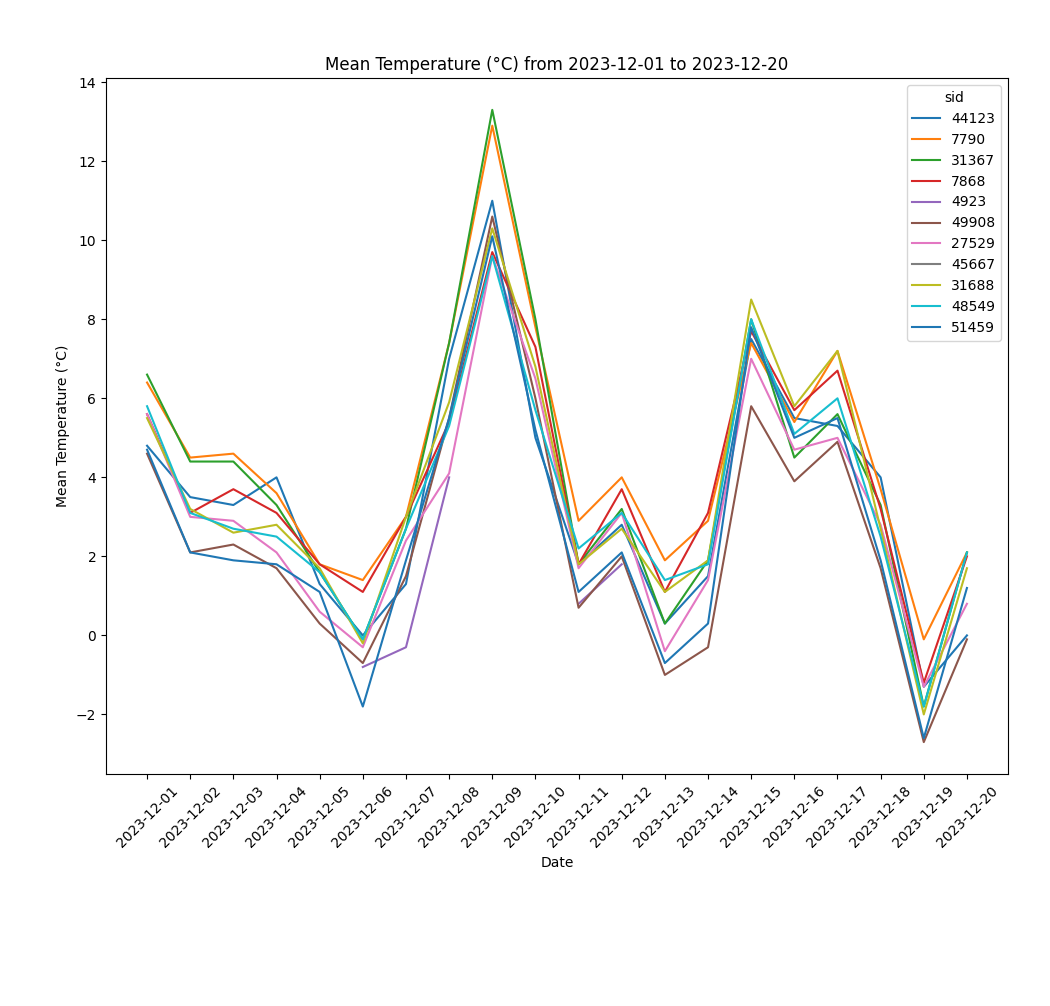
\includegraphics[width=\textwidth]{pic/MD-example.png}
	\caption{Twenty continuous days of mean temperature records for each station, from 2023-12-01 to 2023-12-20}
	\label{Fig:Dataplot}
\end{figure}

One workaround to circumvent this challenge is to use the data from other weather stations geographically nearby. As depicted in Figure~\ref{Fig:Dataplot}, the general trend across all 11 stations within one single GFS grid exhibit remarkable similarity, with differences in mean temperature typically hovering around 2 degrees Celsius. This observation provides a foundation for conjecturing missing data by utilizing available data from neighboring stations. The simpliest approach is to take the average of all available data to impute the missing data. Alternatively, a weighted average can be computed, with weights assigned based on the distance from the target weather station.

In this project, we impute all missing data using the simplest taking average approach. But the following linear regression process only takes data from weather station 44123 as we have the best data quality and least missing values in this weather station.

\subsubsection{Linear Regression}

Linear regression is a commonly used model, which gives a linear relationship between explanatory and the response variable. In our work, the response variable is $Y_t$ and the explanatory variables goes from $X_{t-d}^1, X_{t-d}^2,\ldots,X_{t-d}^p$ at a given time $t$ and previous $d$ days history.

\begin{equation}
	Y_{t} = \beta_0+\sum_{j=1}^p \beta_j X_{t-d}^j + \epsilon_t
\end{equation}

where the coefficient $\beta_j$ are the regression coefficients estimated using a least-squares approach, and $\epsilon$ is the error. We use $d=1$ in our model.

For a large number of variables, in order to obtain a precise estimation, it is necessary to select the most relevant variables. Many methods are available, either forwards or backwards, to retain only a subset of the explanatory variables. Forwards selection starts with an empty list of predictors adding one highly significant predictor at each step until a stopping criterion is reached, whereas backwards selection starts with a full list of predictors eliminating one highly insignificant predictor at each step until a stopping criterion is reached. Omitting the Gaussian assumption, Lasso regression (also called $\mathcal{L}^1$ regularization) may be employed to select the most important predictors by adding a penalty term to the least-squares error (\cite{ISL2}; \cite{Tibshirani1996}). This penalty acts as a constraint favouring a weaker sum of the absolute values of the regression coefficients; this results in some of the coefficients reducing to zero, implying that the corresponding explanatory variable is dropped.

In this project, we trained four seperate models for each quarter of the year and compared the performance between the models.

\section{Results and discussion}

In this section, we present the results obtained from our Linear Regression modeling approach and discuss their implications. We focus on two key aspects: Variable Selection and Cross Validation.

\subsection{Variable Selection}

Variable selection plays a pivotal role in the performance of our Linear Regression models. To ensure optimal model accuracy, we employed rigorous methodologies for selecting the most relevant explanatory variables.

\textbf{Forward and Backward Selection:}

Utilizing forward and backward selection techniques, we systematically identified and retained the most significant predictors for our models. By iteratively adding or removing predictors based on their statistical significance, we aimed to construct parsimonious yet informative models.

\textbf{Lasso Regression (L1 Regularization):}

In addition to traditional variable selection methods, we explored the efficacy of Lasso Regression. By incorporating L1 regularization, we were able to penalize the sum of absolute regression coefficients, leading to the automatic selection of important predictors while discarding irrelevant ones. This approach not only enhanced model interpretability but also improved predictive performance.

\subsection{Cross Validation}

Cross-validation serves as a robust validation technique to assess the generalization capability of our Linear Regression models. We adopted an 8-fold cross-validation strategy to rigorously evaluate model performance across different temporal contexts.

\textbf{Methodology:}

Our cross-validation approach involved partitioning the dataset into eight subsets, with seven years' data utilized for training and one year for testing. Subsequently, we trained four distinct models, each corresponding to a specific quarter of the year (Q1-Q4). This comprehensive approach allowed us to assess the models' ability to capture seasonal variations and temporal dynamics effectively.

\textbf{Results:}

\begin{table}[h]
\centering
\caption{Model Fit Mean Squared Error Results - Station 44123}
\label{tab:CV-result}
\begin{tabular}{@{}lllllllll@{}}
\toprule
\textbf{Model} & \textbf{2016} & \textbf{2017} & \textbf{2018} & \textbf{2019} & \textbf{2020} & \textbf{2021} & \textbf{2022} & \textbf{2023} \\ 
\midrule
Q1        & 2.028            & 2.135            & 1.821            & 2.906            & 1.849            & 1.765            & 2.980            & 2.127            \\
Q2        & 1.190            & 1.637            & 2.275            & 2.287            & 1.912            & 2.280            & 1.353            & 2.281            \\
Q3        & 1.177            & 0.957            & 1.255            & 1.185            & 1.523            & 1.113            & 1.287            & 0.718            \\
Q4        & 1.329            & 1.404            & 1.383            & 1.506            & 1.384            & 1.065            & 1.983            & 0.939            \\ 
\bottomrule
\end{tabular}
\end{table}

The Cross Validation result is shown in Table~\ref{tab:CV-result}. Through cross-validation, we obtained insightful results regarding the predictive performance of our models. By evaluating metrics such as Mean Squared Error (MSE), we gained valuable insights into the models' accuracy and robustness. Additionally, cross-validation facilitated the identification of potential overfitting issues and provided guidance for model refinement and improvement.



\subsection{Discussion}

Figures~\ref{Fig:pred-1} through \ref{Fig:pred-4} depict the model predictions against the true values. The graphs illustrate the accuracy of our predictions relative to the historical weather records. We can see from the graph that our predictionn is very close to the true value.

\begin{figure}[htpb]
	\centering
	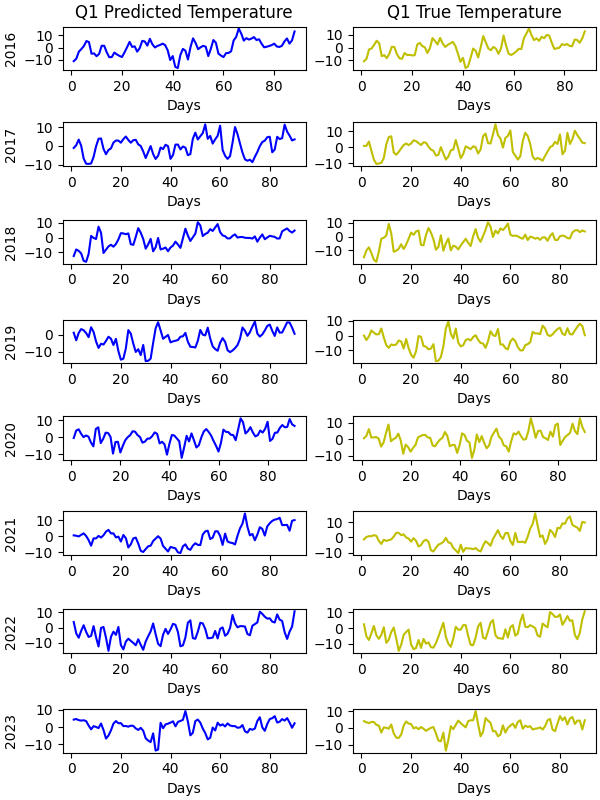
\includegraphics[width=0.8\textwidth]{pic/Predicted-and-Tested-InSeq_1.png}
	\caption{Regression result: January to March}
	\label{Fig:pred-1}
\end{figure}

\begin{figure}[htpb]
	\centering
	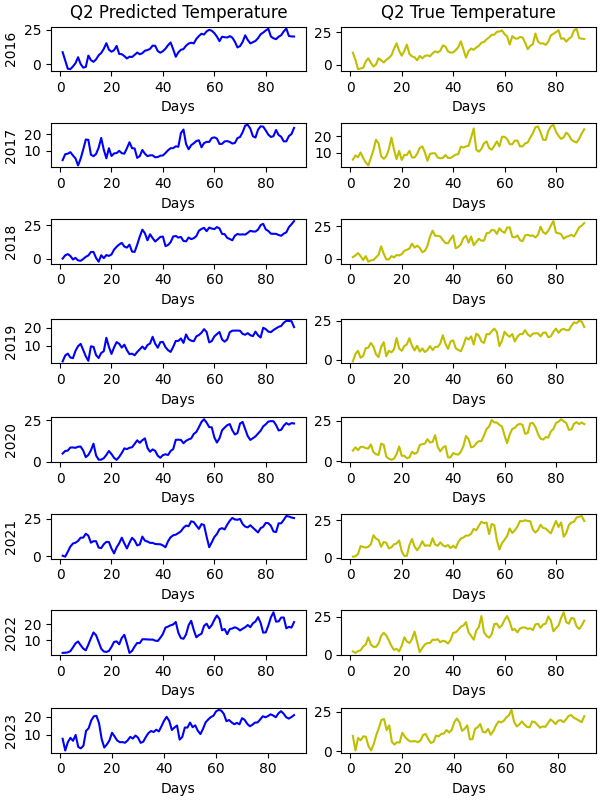
\includegraphics[width=0.8\textwidth]{pic/Predicted-and-Tested-InSeq_2.png}
	\caption{Regression result: April to June}
	\label{Fig:pred-2}
\end{figure}

\begin{figure}[htpb]
	\centering
	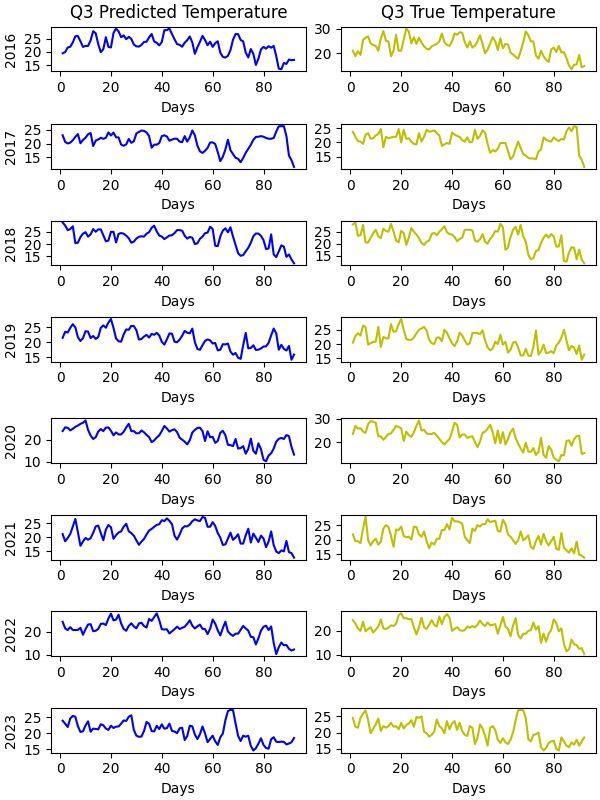
\includegraphics[width=0.8\textwidth]{pic/Predicted-and-Tested-InSeq_3.png}
	\caption{Regression result: July to September}
	\label{Fig:pred-3}
\end{figure}

\begin{figure}[htpb]
	\centering
	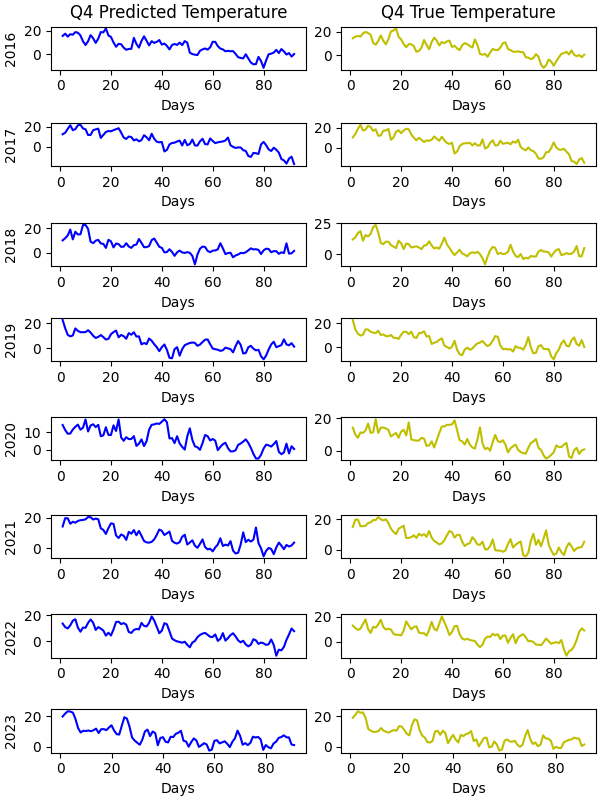
\includegraphics[width=0.8\textwidth]{pic/Predicted-and-Tested-InSeq_4.png}
	\caption{Regression result: October to December}
	\label{Fig:pred-4}
\end{figure}


The results obtained from our Linear Regression models underscore the importance of rigorous variable selection and cross-validation techniques in weather prediction tasks. By selecting relevant variables and validating model performance across diverse temporal contexts, we were able to develop robust and reliable models capable of accurately predicting weather variables.

Moreover, the insights gleaned from our analysis can inform future research endeavors aimed at enhancing the predictive capability of weather forecasting models. By refining variable selection methodologies and adopting advanced validation techniques, we can further improve the accuracy and reliability of weather prediction models, thereby aiding decision-making processes in various sectors.


We evaluate the generalization capability of our model by testing it on a new dataset obtained from weather station 51459. This dataset is not used when we train or validate the model.

\begin{table}[h]
\centering
\caption{Model Fit Mean Squared Error Results: New Station 51459}
\label{tab:model_fit_mse}
\begin{tabular}{@{}lllllllll@{}}
\toprule
\textbf{Model} & \textbf{2016} & \textbf{2017} & \textbf{2018} & \textbf{2019} & \textbf{2020} & \textbf{2021} & \textbf{2022} & \textbf{2023} \\ 
\midrule
Q1        & 2.849            & 1.937            & 2.544            & 2.858            & 1.918            & 1.494            & 2.791            & 1.830            \\
Q2        & 0.921            & 1.401            & 1.331            & 1.198            & 1.154            & 1.041            & 1.436            & 1.052            \\
Q3        & 0.687            & 0.953            & 1.069            & 0.896            & 1.109            & 0.900            & 0.838            & 0.616            \\
Q4        & 1.328            & 1.752            & 1.734            & 1.456            & 1.464            & 1.285            & 1.451            & 1.363            \\ 
\bottomrule
\end{tabular}
\end{table}

The table~\ref{tab:model_fit_mse} presents the Mean Squared Error (MSE) results for four different models evaluated over a span of 8 years from 2016 to 2023. From this table, we can interpret our linear regression result as follows:

\begin{itemize}
\item \textbf{Model performance variation is relatively small:} Each row in the table represents the MSE values for a specific model across different years. Observing that there are some fluctuations in MSE values across years, but overall the MSE values are relative stable. So it's promising that our model's performance over time is consistent.

\item \textbf{Our model performs slightly better at spring and summer:} By analyzing the MSE values, we can see that the model is more stable at Q2 and Q3.

\item \textbf{Temporal Trends:} The MSE values over consecutive years can reveal any temporal trends in model performance. For instance, a gradual increase or decrease in MSE over time may suggest underlying changes in weather patterns or data characteristics that impact model accuracy. In our regressionn results, there is no significant temporal trends.

\end{itemize}


These interpretations can guide further analysis and refinement of the models, ultimately contributing to improved weather prediction accuracy and reliability.


\section{Conclusion}

In conclusion, this study has demonstrated the effectiveness of machine-learning techniques in enhancing air temperature predictions derived from Numerical Weather Prediction (NWP) model outputs. By leveraging historical climatological data and reanalysis products, we have developed robust machine-learning models capable of calibrating NWP model outputs to improve the accuracy of surface temperature estimates.

Through rigorous variable selection, cross-validation, and model evaluation methodologies, we have assessed the performance and generalization capability of the proposed models. Our findings indicate that machine-learning approaches offer promising solutions for addressing inherent biases and inaccuracies present in NWP model outputs, particularly in regions with complex atmospheric dynamics.

The results of our analysis have implications for various applications, including weather forecasting, climate modeling, and environmental management. By improving the accuracy and reliability of surface temperature predictions, our research contributes to the advancement of weather prediction techniques and provides valuable insights for decision-making in sectors such as agriculture, energy, and disaster management.

Moving forward, further research could explore the integration of additional meteorological variables and data sources to enhance the predictive capability of machine-learning models for weather forecasting and climate modeling applications. Additionally, ongoing advancements in machine-learning algorithms and computational techniques offer opportunities for developing more sophisticated models capable of capturing complex atmospheric processes and improving the reliability of weather predictions in diverse geographic regions.

\bibliography{cite}

\end{document}

